%%%%%%%%%%%%%%%%%%%%%%%%%%%%%%%%%%%%%%%%%%%%%%%%%%%555
%From jm and nicolas frame 

  \newcommand{\mEDEA}{

	\begin{itemize}
		\item Chaque agent contient:
		\begin{itemize}
			\item un génome actif, utilisé pour contrôler l'agent,
			\item Une \emph{liste des génomes re\c cus}, utilisée pour stocker les génomes re\c cus pendant une génération,  
		\end{itemize}
		
		\item \`{A} chaque pas de temps, chaque agent :
		\begin{itemize}
			\item émet des copies dont son génome actif,
			\item stocke les génomes re\c cus des agents voisins.
		\end{itemize}
		
		\item \`{A} la fin d'une génération, chaque agent:
		\begin{itemize}
			\item "oublie" son génome actif, 
			\item choisit au hasard un génome parmis les génomes de sa \emph{liste de génomes re\c cus} comme nouveau génome actif et le mute légèrement,
			\item vide sa liste des génomes re\c cus.
		\end{itemize}
	\end{itemize}

}


%------------------------------------------------------------
\begin{frame}{L'algorithme <<mEDEA>>}
\begin{figure}
 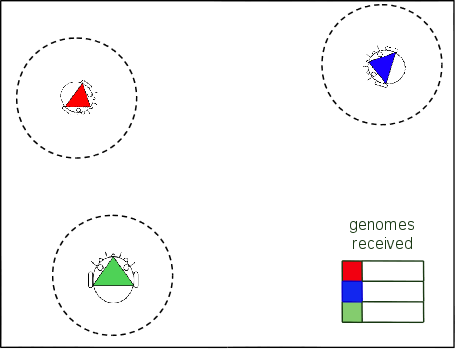
\includegraphics[height=3cm]{images/medea0}
\end{figure}

  \mEDEA

\end{frame}

%------------------------------------------------------------
\begin{frame}{L'algorithme <<mEDEA>>}\addtocounter{framenumber}{-1}
\begin{figure}
 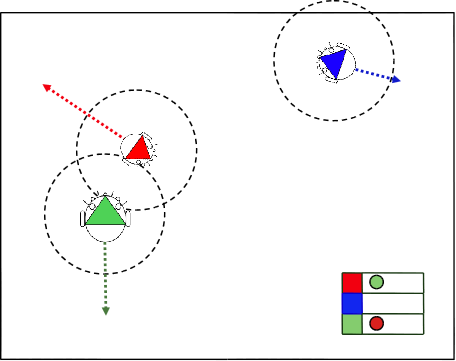
\includegraphics[height=3cm]{images/medea1}
\end{figure}
   \mEDEA
\end{frame}
%------------------------------------------------------------
\begin{frame}{L'algorithme <<mEDEA>>}\addtocounter{framenumber}{-1}
\begin{figure}
 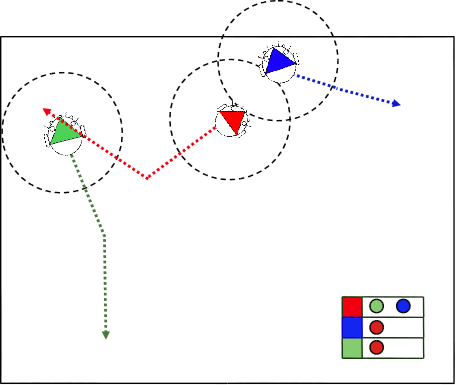
\includegraphics[height=3cm]{images/medea2}
\end{figure}
   \mEDEA
\end{frame}

%------------------------------------------------------------

\begin{frame}{L'algorithme <<mEDEA>>}\addtocounter{framenumber}{-1}
\begin{figure}
 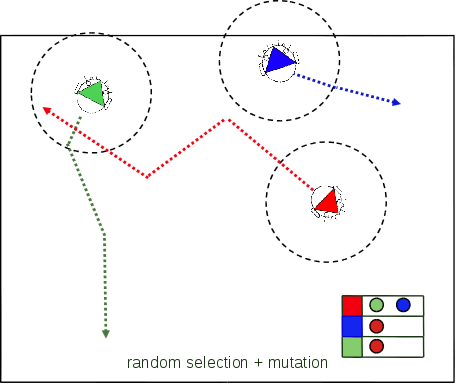
\includegraphics[height=3cm]{images/medea3}
\end{figure}
   \mEDEA
\end{frame}


%%%%%%%%%%%%%%%%%%%%%%%%%%%%%%%%%%


